\section{Teilversuch 2: Drehmoment des Feldes auf eine stromdurchflossene Spule}
	Fehler bei der Winkelmessung $\Delta \alpha = \SI{2}{\degree}$ \\
	Fehler bei der Winkelmessung $\Delta \beta = \SI{1.0}{\degree}$
 	\begin{equation*}
 		\begin{tabu}{l *{10}{r}}
 			\toprule
 			\alpha / \si{\degree} & 0 & 10 & 20 & 30 & 40 & 50 & 60 & 70 & 80 & 90 \\
 			\midrule
			\beta/ \si{\degree} & 295,0 & 315,0 & 337,0 & 358,5 & 377,0 & 395,0 & 413,0 & 425,5 & 437,5 & 449,0 \\
			(\beta - \beta_0)/ \si{\degree} & 0,0 & 20,0 & 42,0 & 63,5 & 82,0 & 100,0 & 118,0 & 130,5 & 142,5 & 154,0 \\
			\varphi / \si{\degree} & 0,0 & -10,0 & -22,0 & -33,5 & -42,0 & -50,0 & -58,0 & -60,5 & -62,5 & -64,0 \\
			\bottomrule
 		\end{tabu}
 	\end{equation*}
	wobei $\varphi = \alpha - (\beta - \beta_0)$.

	Die entsprechende Fehler zur $\sin (\alpha/\si{\degree})$ und $\varphi$ sind wie folgt gegeben:
	\begin{align}
		\Delta \sin (\alpha/\si{\degree}) &= \abs{\cos(\alpha/\si{\degree})}\cdot \frac{\Delta \alpha}{\SI{180}{\degree}} \cdot \pi \\
		\Delta \varphi &= \addquad{\alpha, \beta, \beta_0} = \addquadpure{\SI{2}{\degree}, \SI{1.0}{\degree},\SI{1.0}{\degree}} = \SI{2.5}{\degree}
	\end{align}

	$\varphi$ wurde dann gegen $\sin (\alpha/\si{\degree})$ im \gnuplot{} geplottet und eine Kurveanpassung zur $\varphi = m\sin \alpha + c$ durchgeführt. Die entsprechende Fehler sind direkt im \gnuplot{} berechnet. Siehe Appendix \ref{appdx:gnuplottv2} für die genauer Rechnung.

	Im Experiment war die Markierung für Winkel $\alpha$ wegen des Aufbaus schwer abzulesen. Somit ist der Fehler eher groß und sind hier bei der Kurvenanpassung nicht vernachlässigt.
	\begin{figure}[H]
		\centering
		% GNUPLOT: LaTeX picture with Postscript
\begingroup
  \makeatletter
  \providecommand\color[2][]{%
    \GenericError{(gnuplot) \space\space\space\@spaces}{%
      Package color not loaded in conjunction with
      terminal option `colourtext'%
    }{See the gnuplot documentation for explanation.%
    }{Either use 'blacktext' in gnuplot or load the package
      color.sty in LaTeX.}%
    \renewcommand\color[2][]{}%
  }%
  \providecommand\includegraphics[2][]{%
    \GenericError{(gnuplot) \space\space\space\@spaces}{%
      Package graphicx or graphics not loaded%
    }{See the gnuplot documentation for explanation.%
    }{The gnuplot epslatex terminal needs graphicx.sty or graphics.sty.}%
    \renewcommand\includegraphics[2][]{}%
  }%
  \providecommand\rotatebox[2]{#2}%
  \@ifundefined{ifGPcolor}{%
    \newif\ifGPcolor
    \GPcolortrue
  }{}%
  \@ifundefined{ifGPblacktext}{%
    \newif\ifGPblacktext
    \GPblacktexttrue
  }{}%
  % define a \g@addto@macro without @ in the name:
  \let\gplgaddtomacro\g@addto@macro
  % define empty templates for all commands taking text:
  \gdef\gplbacktext{}%
  \gdef\gplfronttext{}%
  \makeatother
  \ifGPblacktext
    % no textcolor at all
    \def\colorrgb#1{}%
    \def\colorgray#1{}%
  \else
    % gray or color?
    \ifGPcolor
      \def\colorrgb#1{\color[rgb]{#1}}%
      \def\colorgray#1{\color[gray]{#1}}%
      \expandafter\def\csname LTw\endcsname{\color{white}}%
      \expandafter\def\csname LTb\endcsname{\color{black}}%
      \expandafter\def\csname LTa\endcsname{\color{black}}%
      \expandafter\def\csname LT0\endcsname{\color[rgb]{1,0,0}}%
      \expandafter\def\csname LT1\endcsname{\color[rgb]{0,1,0}}%
      \expandafter\def\csname LT2\endcsname{\color[rgb]{0,0,1}}%
      \expandafter\def\csname LT3\endcsname{\color[rgb]{1,0,1}}%
      \expandafter\def\csname LT4\endcsname{\color[rgb]{0,1,1}}%
      \expandafter\def\csname LT5\endcsname{\color[rgb]{1,1,0}}%
      \expandafter\def\csname LT6\endcsname{\color[rgb]{0,0,0}}%
      \expandafter\def\csname LT7\endcsname{\color[rgb]{1,0.3,0}}%
      \expandafter\def\csname LT8\endcsname{\color[rgb]{0.5,0.5,0.5}}%
    \else
      % gray
      \def\colorrgb#1{\color{black}}%
      \def\colorgray#1{\color[gray]{#1}}%
      \expandafter\def\csname LTw\endcsname{\color{white}}%
      \expandafter\def\csname LTb\endcsname{\color{black}}%
      \expandafter\def\csname LTa\endcsname{\color{black}}%
      \expandafter\def\csname LT0\endcsname{\color{black}}%
      \expandafter\def\csname LT1\endcsname{\color{black}}%
      \expandafter\def\csname LT2\endcsname{\color{black}}%
      \expandafter\def\csname LT3\endcsname{\color{black}}%
      \expandafter\def\csname LT4\endcsname{\color{black}}%
      \expandafter\def\csname LT5\endcsname{\color{black}}%
      \expandafter\def\csname LT6\endcsname{\color{black}}%
      \expandafter\def\csname LT7\endcsname{\color{black}}%
      \expandafter\def\csname LT8\endcsname{\color{black}}%
    \fi
  \fi
    \setlength{\unitlength}{0.0500bp}%
    \ifx\gptboxheight\undefined%
      \newlength{\gptboxheight}%
      \newlength{\gptboxwidth}%
      \newsavebox{\gptboxtext}%
    \fi%
    \setlength{\fboxrule}{0.5pt}%
    \setlength{\fboxsep}{1pt}%
\begin{picture}(8640.00,5760.00)%
    \gplgaddtomacro\gplbacktext{%
      \csname LTb\endcsname%%
      \put(814,704){\makebox(0,0)[r]{\strut{}$-70$}}%
      \put(814,1332){\makebox(0,0)[r]{\strut{}$-60$}}%
      \put(814,1960){\makebox(0,0)[r]{\strut{}$-50$}}%
      \put(814,2588){\makebox(0,0)[r]{\strut{}$-40$}}%
      \put(814,3215){\makebox(0,0)[r]{\strut{}$-30$}}%
      \put(814,3843){\makebox(0,0)[r]{\strut{}$-20$}}%
      \put(814,4471){\makebox(0,0)[r]{\strut{}$-10$}}%
      \put(814,5099){\makebox(0,0)[r]{\strut{}$0$}}%
      \put(946,484){\makebox(0,0){\strut{}$0,1$}}%
      \put(1714,484){\makebox(0,0){\strut{}$0,2$}}%
      \put(2482,484){\makebox(0,0){\strut{}$0,3$}}%
      \put(3250,484){\makebox(0,0){\strut{}$0,4$}}%
      \put(4018,484){\makebox(0,0){\strut{}$0,5$}}%
      \put(4787,484){\makebox(0,0){\strut{}$0,6$}}%
      \put(5555,484){\makebox(0,0){\strut{}$0,7$}}%
      \put(6323,484){\makebox(0,0){\strut{}$0,8$}}%
      \put(7091,484){\makebox(0,0){\strut{}$0,9$}}%
      \put(7859,484){\makebox(0,0){\strut{}$1$}}%
    }%
    \gplgaddtomacro\gplfronttext{%
      \csname LTb\endcsname%%
      \put(209,2901){\rotatebox{-270}{\makebox(0,0){\strut{}Torsionswinkel $\phi$ ($\si{\degree}$)}}}%
      \put(4594,154){\makebox(0,0){\strut{}$\sin(\alpha/\si{\degree})$}}%
      \csname LTb\endcsname%%
      \put(7256,4893){\makebox(0,0)[r]{\strut{}$-64,51852I + -0,14015$}}%
      \csname LTb\endcsname%%
      \put(7256,4607){\makebox(0,0)[r]{\strut{}Messpunkte}}%
      \csname LTb\endcsname%%
      \put(4594,5429){\makebox(0,0){\strut{}Torsionswinkel $\phi$ gegen $\sin(\alpha/\si{\degree})$}}%
    }%
    \gplbacktext
    \put(0,0){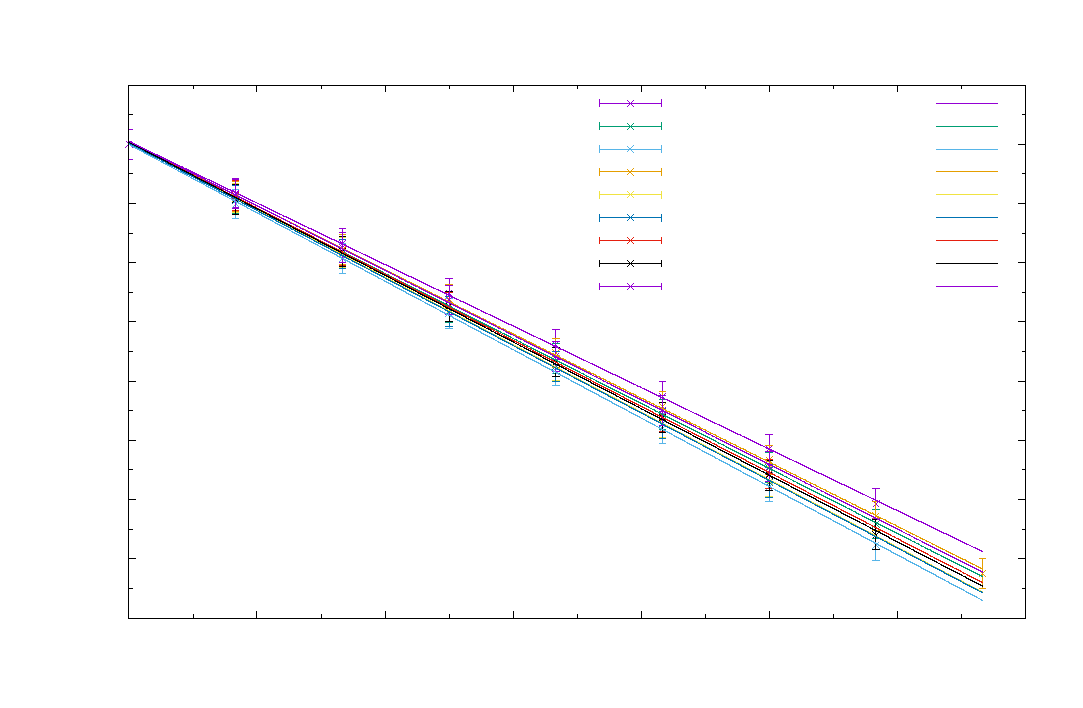
\includegraphics[width={432.00bp},height={288.00bp}]{tv2-plot}}%
    \gplfronttext
  \end{picture}%
\endgroup

		\caption{\centering Drehmoment auf stromdurchflossene Spule \captionbr $\chi^2_{\text{red}} = \num{0.163741} \implies$ Gute Anpassung}
		\label{fig:tvtwo-plot}
		\vspace{-1em}
	\end{figure}
	Als Endergebnis erhalten wir:
	\begin{equation*}
		\begin{tabu}{lll}
			\toprule
			\text{Variable} & \text{Wert} & \text{Gerundet} \\
			\midrule
			m & \SI{-64.519(1445)}{\degree} & \SI{-64.5(15)}{\degree}\\
			c & \SI{-0.140(1145)}{\degree} & \SI{-0.1(12)}{\degree} \\
			\bottomrule
		\end{tabu}
	\end{equation*}
	$c$ ist der Ordinateabschnitt und $0$ liegt tatsächlich im Fehlerintervall von $c$, also liegen die Messpunkte im Rahmen der Fehlergrenzen auf einer durch den Nullpunkt gehenden Geraden.

	Aus der gute Kurvenanpassung folgt also, dass die Messergebnisse mit der Theorie übereinstimmt. 